Putting it all together, here is my design of a single-layer peceptron:

\begin{figure}[H]
  \centering
  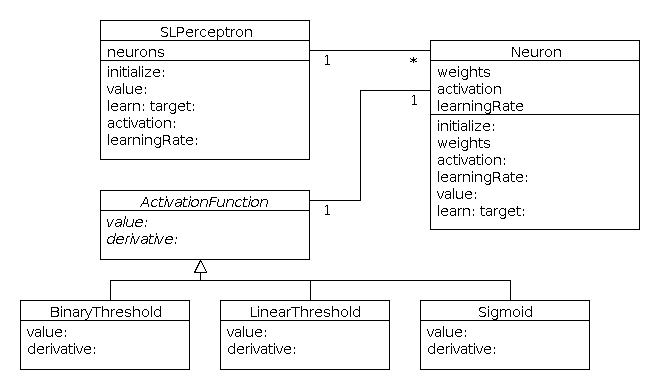
\includegraphics[width=0.9\linewidth]{slp}
  \caption{Object-oriented design of a single-layer perceptron}
  \label{fig:slp2}
\end{figure}

\subsection{Neuron class}
\begin{lstlisting}
Object subclass: #Neuron
   instanceVariableNames: 'weights activation learningRate'
   classVariableNames: ''
   package: 'NeuralNetwork'
\end{lstlisting}

The weights are initialized with random numbers in range [0, 1]. I’m not sure if this is a good range, but on simple examples it works just fine.

BinaryThreshold is a default activation function and the default learning rate is 0.1. These parameters can be changed using the accessors activation: and learningRate:.

\begin{lstlisting}
initialize: inputSize
   "Creates a weight vector and initializes it with random values. Assigns default values to activation and learning rate"

   activation := BinaryThreshold new.
   learningRate := 0.1.
 
   weights := DhbVector new: (inputSize + 1).
 
   1 to: (inputSize + 1) do: [ :i |
      weights at: i put: (1 / (10 atRandom))].
   ^ self
\end{lstlisting}

We will also need to prepend 1 as a bias unit to every input vector.

\begin{lstlisting}
prependBiasToInput: inputVector
   "this method prepends 1 to input vector for a bias unit"
 
   ^ (#(1), inputVector) asDhbVector.
\end{lstlisting}

According to “Numerical Methods” book, each function should implement the value: method. I want to emphasize that from the mathematical point of view neuron is a function.

Though the inner representation uses DhbVector, I want a user to write something like perceptron value: \#(1 0). instead of perceptron value: \#(1 0) asDhbVector.

\begin{lstlisting}
value: inputVector
   "Takes a vector of inputs and returns the output value"
 
   | inputDhbVector |
   inputDhbVector := self prependBiasToInput: inputVector.
   ^ activation value: (weights * inputDhbVector).
\end{lstlisting}

We need accessors for setting the learning rate an activation. I also added a simple accessor for weights for debugging purposes. All these accessors are trivial, so I will not put the code here.

And of course, the perceptron learning rule.

\begin{lstlisting}
learn: inputVector target: target
   "Applies the perceptron learning rule after looking at one training example"
 
   | input output error delta |
   output := self value: inputVector.
   error := target - output.
 
   input := self prependBiasToInput: inputVector.
  
   delta := learningRate * error * input * 
      (activation derivative: weights * input).
\end{lstlisting}
      
\subsection{SLPerceptron class}
Single-layer perceptron (according to my design) is a container of neurons. The only instance variable it has is the neurons array.

\begin{lstlisting}
Object subclass: #SLPerceptron
   instanceVariableNames: 'neurons'
   classVariableNames: ''
   package: 'NeuralNetwork'
\end{lstlisting}

To create an instance of SLPerceptron we need to specify the size of the input vector and the number of classes which equals to the number of neurons in our perceptron (multiclass classification).

\begin{lstlisting}
initialize: inputSize classes: outputSize
   "Creates an array of neurons"
   neurons := Array new: outputSize.
 
   1 to: outputSize do: [ :i |
      neurons at: i put: (Neuron new initialize: inputSize). ]
\end{lstlisting}

The output of a single-layer perceptron is a vector of scalar outputs from each neuron in the layer.

\begin{lstlisting}
value: input
   "Returns the vector of outputs from each neuron"
   | outputVector |
 
   outputVector := Array new: (neurons size).
 
   1 to: (neurons size) do: [ :i |
      outputVector at: i put: ((neurons at: i) value: input) ].
 
   ^ outputVector
\end{lstlisting}

If we ask SLPerceptron to learn, he will pass that request to all his neurons (basically, SLPerceptron is just a container of neurons that provides an interface for manipulating them).

\begin{lstlisting}
learn: input target: output
   "Trains the network (perceptron) on one (in case of online learning) or multiple (in case of batch learning) input/output pairs"

  1 to: (neurons size) do: [ :i |
     (neurons at: i) learn: input target: (output at: i) ].
\end{lstlisting}
